\documentclass[12pt, a4paper]{article}
\usepackage[margin=1in]{geometry}

% text
\usepackage{amsthm, amsmath, amssymb}
\tolerance=1
\emergencystretch=\maxdimen
\hyphenpenalty=10000
\hbadness=10000
\parindent=0pt % remove indentation after figures
\usepackage{setspace} 
\onehalfspacing 
\raggedbottom % removes space between paragrafs

% 
\usepackage{paracol}

% grafics
\usepackage{graphicx}
\graphicspath{ {./img/} }
\usepackage{float}

% title
\title{\vspace{-0.5cm}Praktikum Regelungstechnik: Frequenzganganalyse\vspace{-0.5cm}}
\author{Robin Seidel \& Ben Müller}
\date{06.01.2025}


% === Content ===
\begin{document}

\maketitle

\newpage
\section*{Versuchsvorbereitung}
Das Kolloquium zur Versuchsvorbereitung erfolgt mündlich in der Gruppe, ohne Unter-
lagen.

\begin{enumerate}
    \item Was ist ein Frequenzgang?
    \vspace{-16pt}\paragraph{Antwort:} ist das Übertragungsverhalten eines Systems bezüglich seiner Phase ($\phi$) und Amplitude ($A$) in Abhängigkeit der Veränderung der Frequenz.
    \[ y(t) = A_{1} \cdot \sin(\omega t + \phi_{1})  \rightarrow System: G(s) \rightarrow y(t) = A_{2} \cdot \sin(\omega t + \phi_{2})\]
    \begin{paracol}{2}
        \begin{figure}[H]
            \centering
            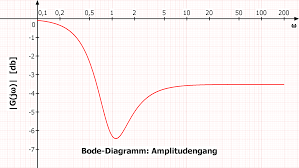
\includegraphics[width=0.45\textwidth]{amplitudengang.png}
            \caption{Beispiel Amplitudengang}
        \end{figure}
    \switchcolumn
        \begin{figure}[H]
            \centering
            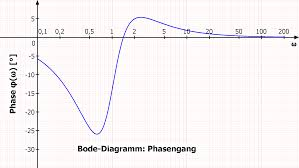
\includegraphics[width=0.45\textwidth]{phasengang.jpg}
            \caption{Beispiel Phasengang}
        \end{figure}
    \end{paracol}

    \item Was ist ein Bode-Diagramm? Weshalb werden die Abszissen darin logarithmisch dargestellt?
    \vspace{-16pt}\paragraph{Antwort (Bode-Diagramm):} Es ist die Darstellung der Amplitudenveränderung und Phasenverschiebung in Abhängigkeit von der Frequenz.
    \vspace{-16pt}\paragraph{Antwort (logarithmischre Abszisse):} Um in Reihe geschaltete Übertragungsglieder einfacher überlagern/addieren zu können wird der Amplitudengang logarithmisch dargestellt.
    
    \item Wozu dient die Frequenzganganalyse? Welche Eigenschaften eines dynamischen Systems lassen sich aus seinem Frequenzgang ableiten?
    \vspace{-16pt}\paragraph{Antwort:} Es lässt sich abschätzen wie schnell und genau ein System auf Veränderungen der Ausgangparameter reagiert. Zusätzlich dient es zur Bestimmung der Stabilität, Resonanz, Bandbreite und Dynamik des Systems.
    
    \item Worin unterscheidet sich eine Asymptote von einer Tangente?
    \vspace{-16pt}\paragraph{Antwort:} Eine Asymptote gibt an welchen Wert sich eine Funktion annähert, eine Tangente hingegen gibt an welchen Punkt eine Funktion schneidet.
    
    \item Wie ermittelt man die Verstärkung und die Knickfrequenzen im Amplitudengang? Welche konkreten Anstiege (db/Dekade) dürfen Asymptoten im Amplitudengang haben?
    \vspace{-16pt}\paragraph{Antwort (Verstärkung):} \mbox{} \\
    Bsp PT1:: $G(s) = \frac{K}{1+T \cdot s} $; $K=$ Verstärkungsfaktor \\
    $ K|_{dB} = 20 \log_{10}(K) $
    \vspace{-16pt}\paragraph{Antwort (Knickfrequenzen):} Inverse Zeitkonstante $= \omega_0 = T^{-1}$ 
    \vspace{-16pt}\paragraph{Antwort (Anstieg db/Dekade):} Übertragungsglieder haben alle eigene Anstiege, Asymptoten hingegen sollten einen Anstieg von $0dB/Dekade$ aufweisen.
    
    \item Wie lassen sich Kennwerte und die Stabilität eines Systems aus seiner Ortskurve bestimmen?
    \vspace{-16pt}\paragraph{Antwort (Kennwerte):} Die länge des Zeigers ist äquivalent zum Betrag des Übertragungsglieds. Der Winkel/ das Arqument des Zeigers repräsentiert die Phasenverschiebung.
    \vspace{-16pt}\paragraph{Antwort (Stabilität):} Wenn die Verstärkung kleiner 1 ist ist das System stabiel.
    \begin{figure}[H]
        \centering
        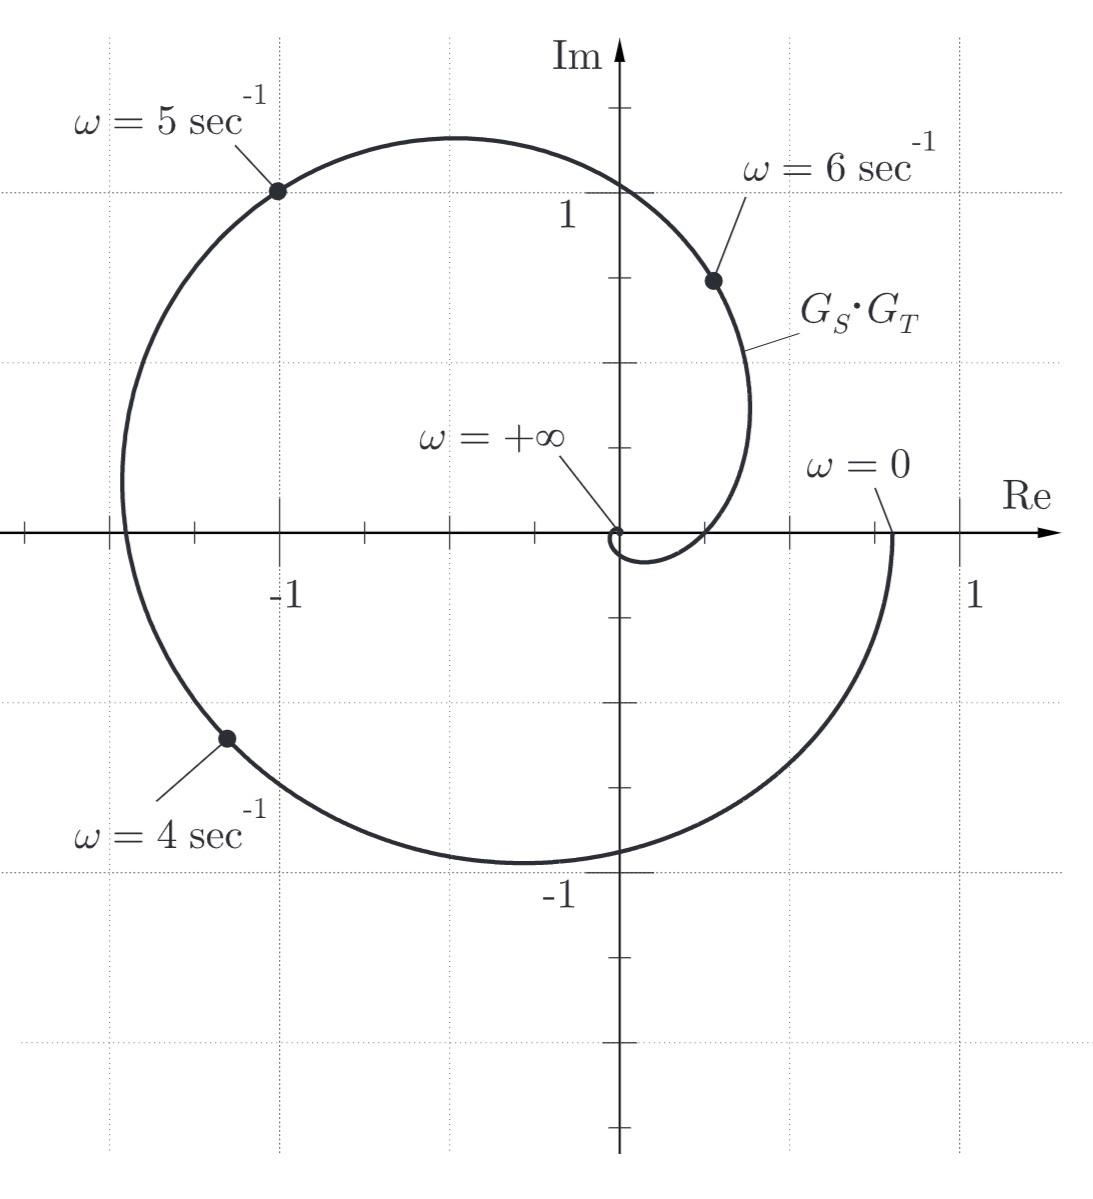
\includegraphics[width=0.6\textwidth]{nyquist_kriteriumjpg.jpg}
        \caption{Beispiel Niquist Kriterium}
    \end{figure}

\end{enumerate}

\hrule
\paragraph{Wichtig:} Für den Versuch sind mitzubringen: Taschenrechner, Polarkoordinatenpapier
und halblogarithmisch geteiltes Papier.

\end{document}